\documentclass[a4paper]{article}
%\usepackage[singlespacing]{setspace}
\usepackage[onehalfspacing]{setspace}
%\usepackage[doublespacing]{setspace}
\usepackage{geometry} % Required for adjusting page dimensions and margins
\usepackage{amsmath,amsfonts,stmaryrd,amssymb,mathtools,dsfont} % Math packages
\usepackage{tabularx}
\usepackage{colortbl}
\usepackage{listings}
\usepackage{amsmath}
\usepackage{amssymb}
\usepackage{amsthm}
\usepackage{enumerate}
\usepackage{enumitem}
\usepackage{subcaption}
\usepackage{float}
\usepackage[table,xcdraw]{xcolor}
\usepackage{tikz-qtree}
\usepackage{tikz}
\usepackage{pgfplots}
\pgfplotsset{compat=1.17}
\usepackage{forest}
\usepackage{changepage,titlesec,fancyhdr} % For styling Header and Titles
\pagestyle{fancy}
\renewcommand{\headrulewidth}{0.5pt} % Linienbreite anpassen, falls gewünscht
\renewcommand{\headrule}{
    \makebox[\textwidth]{\rule{1.0\textwidth}{0.5pt}} 
}
\usepackage{amsmath}
\pagestyle{fancy}
\usepackage{diagbox}
\usepackage{xfrac}

\usepackage{enumerate} % Custom item numbers for enumerations

\usepackage[ruled]{algorithm2e} % Algorithms

\usepackage[framemethod=tikz]{mdframed} % Allows defining custom boxed/framed environments

\usepackage{listings} % File listings, with syntax highlighting
\lstset{
	basicstyle=\ttfamily, % Typeset listings in monospace font
}

\usepackage[ddmmyyyy]{datetime}

\geometry{
	paper=a4paper, % Paper size, change to letterpaper for US letter size
	top=3cm, % Top margin
	bottom=3cm, % Bottom margin
	left=2.5cm, % Left margin
	right=2.5cm, % Right margin
	headheight=25pt, % Header height
	footskip=1.5cm, % Space from the bottom margin to the baseline of the footer
	headsep=1cm, % Space from the top margin to the baseline of the header
	%showframe, % Uncomment to show how the type block is set on the page
}
\lhead{Analysis und Numerik\\Sommersemester 2025}
\chead{\bfseries{\vspace{0.5\baselineskip}Übungsblatt 5}}
\rhead{Lienkamp, 8128180\\Werner, 7987847}
\fancyheadoffset[R]{0cm}

\begin{document}
\setcounter{section}{5}
\subsection{Votieraufgabe}
Sei $a_n)_n \subset \mathbb{R}$ eine reelle Folge.
\begin{enumerate}[label=(\alph*)]
    \item Zeigen Sie, dass wenn
    \[\lim\limits_{n\to\infty}\sqrt[n]{|a_n|}=L<1,\]
    dann konvergiert die Reihe $\sum\limits^\infty_{n=0}a_n$ absolut.
    \item Geben Sie ein Beispiel für $L = 1$ an, sodass die Reihe $\sum\limits^\infty_{n=0}a_n$ an nicht konvergiert.
\end{enumerate}
\subsection{Multiple Choice}
Kreuzen Sie bei den folgenden Fragen jeweils die zutreende Antwort an. Korrekte Kreuze bringen +0.5 Punkte. Falsche Kreuze -0.5 Punkte. Sie bekommen auf diese Aufgabe mindestens 0 Punkte.\\
Seien $(a_n)_n, (b_n)_n, (c_n)_n, (d_n)_n \subset \mathbb{R}$ reelle Folgen.
\begin{enumerate}[label=(\alph*)]
    \item Falls $(a_n)_n$ eine Nullfolge ist, so konvergiert für jede beliebige Folge $(b_n)_n$ mit $b_n > nb_{n+1} + a_n$ das Produkt $(a_nb_n)_n \subset \mathbb{R}$.
    \begin{flushright}
        wahr $\square\quad$ falsch $\boxtimes$
    \end{flushright}
    \item Sei $a_n \in O(c_n)$ und $b_n \in O(d_n)$ für $n\to\infty$. Dann gilt:
    \[(a_n+b_n)\in O(c_n+d_n)\quad \text{ für } n\to\infty\]
    \begin{flushright}
        wahr $\boxtimes\quad$ falsch $\square$
    \end{flushright}
    \item Für $(a_n) \in O\left(\frac{1}{n^2}\right)$ ist $(a_n)\in o\left(\frac{1}{n}\right)$ für $n\to\infty$.
    \begin{flushright}
        wahr $\boxtimes\quad$ falsch $\square$
    \end{flushright}
    \item Für $(a_n) \in o\left(\frac{1}{n}\right)$ ist $(a_n) \in O\left(\frac{1}{n^2}\right)$ für $n\to\infty$.   \begin{flushright}
        wahr $\square\quad$ falsch $\boxtimes$
    \end{flushright}
\end{enumerate}
\subsection{Rechenaufgabe}
Ein - zugegeben etwas primitiver - Rechner stellt reelle Zahlen im Gleitkommaformat mit einem Byte dar. Bei der (nomarlisierten) Zahlendarstellung werden 1 Bit für das Vorzeichen, 4 Bits für die Mantisse und 3 Bits für den Exponenten bei einem Bias von 3 verwendet. Bestimmen Sie die Gleitkommadarstellung
\[(-1)^S(1+M\cdot 2^{-4})2^{E-3}\]
der Zahlen und tragen Sie diese in \textbf{Binärdarstellung} in das entsprechende Kästchen. Bitte geben Sie nur die Endergebnisse an. Korrekte Lösungen bringen +0.5 Punkte, falsche Lösungen 0 Punkte.\\\\
\fbox{\parbox{\linewidth}{
\[-1 = \frac{1|0000|011}{S\quad M\quad E\quad}\]
}}\vspace*{5mm}
\fbox{\parbox{\linewidth}{
\[0.125 = \frac{0|0000|000}{S\quad M\quad E\quad}\]
}}\vspace*{5mm}
\fbox{\parbox{\linewidth}{
\[2.5 = \frac{0|0100|100}{S\quad M\quad E\quad}\]
}}\vspace*{5mm}
\fbox{\parbox{\linewidth}{
\[-1.25 = \frac{1|0100|011}{S\quad M\quad E\quad}\]
}}\vspace*{5mm}
\subsection{Schriftliche Aufgabe}
Unser Ein-Byte-Rechner soll weiterhin mit 1 Bit für das Vorzeichen, 4 Bits für die Mantisse und 3 Bits für den Exponenten bei einem Bias von 3 ausgestattet sein.
\begin{enumerate}[label=(\alph*)]
    \item Wie viele verschiedene Zahlen können in diesem Gleitkomma-Format dargestellt werden?\\
    Es können $2^8 = 256$ verschiedene Zahlen dargestellt werden
    \item Geben sie $x_{max}$, $x_{min}$, sowie das betragliche Minimum $x_{minabs}$ an.\\
    $x_{max}=31$\\
    $x_{min}=-31$\\
    $x_{minabs}=0,125$
    \item Skizzieren (bzw. plotten) sie alle darstellbaren Zahlen auf einer Zahlengeraden.\\
    \begin{figure}[h!]
\centering
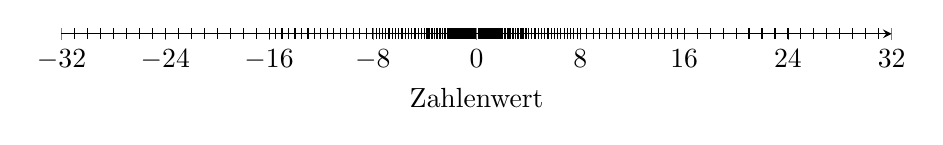
\begin{tikzpicture}
    \begin{axis}[
        width=\textwidth,
        height=5cm,
        axis y line=none,
        axis x line=bottom,
        xmin=-32,
        xmax=32,
        ymin=0,
        ymax=1,
        xtick={-32,-24,-16,-8,0,8,16,24,32},
        xlabel={Zahlenwert},
        ytick=\empty,
    ]

    % Alle darstellbaren positiven Werte
    \addplot[
        only marks,
        mark=|,
    ]
    coordinates {
        % Positive Werte
        (0.125,0) (0.1328125,0) (0.140625,0) (0.1484375,0)
        (0.15625,0) (0.1640625,0) (0.171875,0) (0.1796875,0)
        (0.1875,0) (0.1953125,0) (0.203125,0) (0.2109375,0)
        (0.21875,0) (0.2265625,0) (0.234375,0) (0.2421875,0)

        (0.25,0) (0.265625,0) (0.28125,0) (0.296875,0)
        (0.3125,0) (0.328125,0) (0.34375,0) (0.359375,0)
        (0.375,0) (0.390625,0) (0.40625,0) (0.421875,0)
        (0.4375,0) (0.453125,0) (0.46875,0) (0.484375,0)

        (0.5,0) (0.53125,0) (0.5625,0) (0.59375,0)
        (0.625,0) (0.65625,0) (0.6875,0) (0.71875,0)
        (0.75,0) (0.78125,0) (0.8125,0) (0.84375,0)
        (0.875,0) (0.90625,0) (0.9375,0) (0.96875,0)

        (1.0,0) (1.0625,0) (1.125,0) (1.1875,0)
        (1.25,0) (1.3125,0) (1.375,0) (1.4375,0)
        (1.5,0) (1.5625,0) (1.625,0) (1.6875,0)
        (1.75,0) (1.8125,0) (1.875,0) (1.9375,0)

        (2.0,0) (2.125,0) (2.25,0) (2.375,0)
        (2.5,0) (2.625,0) (2.75,0) (2.875,0)
        (3.0,0) (3.125,0) (3.25,0) (3.375,0)
        (3.5,0) (3.625,0) (3.75,0) (3.875,0)

        (4.0,0) (4.25,0) (4.5,0) (4.75,0)
        (5.0,0) (5.25,0) (5.5,0) (5.75,0)
        (6.0,0) (6.25,0) (6.5,0) (6.75,0)
        (7.0,0) (7.25,0) (7.5,0) (7.75,0)

        (8.0,0) (8.5,0) (9.0,0) (9.5,0)
        (10.0,0) (10.5,0) (11.0,0) (11.5,0)
        (12.0,0) (12.5,0) (13.0,0) (13.5,0)
        (14.0,0) (14.5,0) (15.0,0) (15.5,0)

        (16.0,0) (17.0,0) (18.0,0) (19.0,0)
        (20.0,0) (21.0,0) (22.0,0) (23.0,0)
        (24.0,0) (25.0,0) (26.0,0) (27.0,0)
        (28.0,0) (29.0,0) (30.0,0) (31.0,0)
    };

    % Negative Spiegelung
    \addplot[
        only marks,
        mark=|, 
    ]
    coordinates {
        (-0.125,0) (-0.1328125,0) (-0.140625,0) (-0.1484375,0)
        (-0.15625,0) (-0.1640625,0) (-0.171875,0) (-0.1796875,0)
        (-0.1875,0) (-0.1953125,0) (-0.203125,0) (-0.2109375,0)
        (-0.21875,0) (-0.2265625,0) (-0.234375,0) (-0.2421875,0)

        (-0.25,0) (-0.265625,0) (-0.28125,0) (-0.296875,0)
        (-0.3125,0) (-0.328125,0) (-0.34375,0) (-0.359375,0)
        (-0.375,0) (-0.390625,0) (-0.40625,0) (-0.421875,0)
        (-0.4375,0) (-0.453125,0) (-0.46875,0) (-0.484375,0)

        (-0.5,0) (-0.53125,0) (-0.5625,0) (-0.59375,0)
        (-0.625,0) (-0.65625,0) (-0.6875,0) (-0.71875,0)
        (-0.75,0) (-0.78125,0) (-0.8125,0) (-0.84375,0)
        (-0.875,0) (-0.90625,0) (-0.9375,0) (-0.96875,0)

        (-1.0,0) (-1.0625,0) (-1.125,0) (-1.1875,0)
        (-1.25,0) (-1.3125,0) (-1.375,0) (-1.4375,0)
        (-1.5,0) (-1.5625,0) (-1.625,0) (-1.6875,0)
        (-1.75,0) (-1.8125,0) (-1.875,0) (-1.9375,0)

        (-2.0,0) (-2.125,0) (-2.25,0) (-2.375,0)
        (-2.5,0) (-2.625,0) (-2.75,0) (-2.875,0)
        (-3.0,0) (-3.125,0) (-3.25,0) (-3.375,0)
        (-3.5,0) (-3.625,0) (-3.75,0) (-3.875,0)

        (-4.0,0) (-4.25,0) (-4.5,0) (-4.75,0)
        (-5.0,0) (-5.25,0) (-5.5,0) (-5.75,0)
        (-6.0,0) (-6.25,0) (-6.5,0) (-6.75,0)
        (-7.0,0) (-7.25,0) (-7.5,0) (-7.75,0)

        (-8.0,0) (-8.5,0) (-9.0,0) (-9.5,0)
        (-10.0,0) (-10.5,0) (-11.0,0) (-11.5,0)
        (-12.0,0) (-12.5,0) (-13.0,0) (-13.5,0)
        (-14.0,0) (-14.5,0) (-15.0,0) (-15.5,0)

        (-16.0,0) (-17.0,0) (-18.0,0) (-19.0,0)
        (-20.0,0) (-21.0,0) (-22.0,0) (-23.0,0)
        (-24.0,0) (-25.0,0) (-26.0,0) (-27.0,0)
        (-28.0,0) (-29.0,0) (-30.0,0) (-31.0,0)
    };

    \end{axis}
\end{tikzpicture}
\end{figure}
    \item Bestimmen sie den maximalen absoluten und relativen Rundungsfehler in [$x_{minabs}$, $x_{max}$].\\
    Ab $\pm 16$ kann man die Zahlen nur in 1-er Schritten erreichen. Der größte absolute Fehler liegt also bei 16,5 mit einem Abstand von 0,5 zu den nächsten maschinell erreichbaren Zahlen: $x_{max}=0,5$.(maximaler absoluter Rundungsfehler)\\
    Der relative Rundungsfehler zwischen 16 und 16,5 von 0,5 berechnet sich zu $\frac{16,5-16}{16,5}=\frac{1}{33}$, alle relativen Rundungsfehler bei betraglich größeren Zahlen wird anteilig kleiner, wir vergleichen also mit dem relativen Rundungsfehler zwischen den beiden kleinsten positiven Werten, die berechnen werden können $\frac{\frac{34}{256}-\frac{33}{256}}{\frac{33}{256}}=\frac{1}{33}$.\\
    Den relativen Rundungsfehler zwischen 0,125 und -0,125 können wir nicht berechnen, da wir hierbei durch 0 teilen müssten und das nicht zulässig ist.\\
    Der maximale relative Rundungsfehler liegt somit bei $\frac{1}{33}$.
    \end{enumerate}
\end{document}
